\documentclass[lang = zh , final , oneside , openany , titlepage , zihao = -4 , linespread = 1.3 , baselineskip = false , cjk-font = windows , text-font = newtx , math-font = newtx]{sjtureport}

\usepackage{amsmath}
\usepackage{amsthm}
\usepackage[hidelinks]{hyperref}%目录超链接并隐藏
\usepackage{graphicx}%图片路径支持
\graphicspath{./figures/}%图片路径
\DeclareGraphicsExtensions{.pdf,.eps,.png,.jpg,.jpeg} % 扩展图片格式
\usepackage{gbt7714}
\bibliographystyle{gbt7714-numerical}
\usepackage{booktabs} % 表格支持
\usepackage{longtable} % 表格支持
%\usepackage{subcaption}%小标题支持

%\sjtusetup
%{
%  info =
%  {
%    zh/title = {上海交通大学学位论文模板示例文档},
%    en/title = {A Sample Document for SJTU Thesis Template},
%    zh/author = {某某},
%    en/author = {Mo Mo},
%  },
%
%  style =
%  {
%    float-num-sep = {-},
%  },
%
%  name =
%  {
%    achv = {攻读学位期间完成的论文},
%  },
%}

\title{数学必修一讲义}
%\author{某某}
%\subject{XX期末课程论文}
%\keywords{上海交大, 饮水思源, 爱国荣校}

\begin{document}

\maketitle

\setcounter{page}{1}  % 将页码设置为1
\pagestyle{plain}     % 设置为普通页码样式
\tableofcontents

%\begin{abstract}
%本模板是上海交通大学本科生课程论文、学位论文、学术报告等文档的LaTeX模板,旨在帮助学生快速上手LaTeX排版。
%\end{abstract}

\newpage
\setcounter{page}{1}  % 将页码设置为1
\pagestyle{plain}     % 设置为普通页码样式
\chapter{集合与常用逻辑用语}
\section{集合的概念}
\subsection{集合的定义}

\begin{itemize}
    \item 元素(element):研究的对象、
    \item 集合(set):元素的总体
\end{itemize}

\subsection{集合的性质}

\begin{enumerate}
    \item 确定性:集合的元素是确定的,不能模糊不清。
    \item 无序性:集合的元素没有顺序,元素的排列顺序不影响集合的性质。
    \item 无重复性:集合中的元素不能重复出现,每个元素只能出现一次。
\end{enumerate}

若元素 $a$ 在集合 $A$ 内,我们称 $a$ 属于集合 $A$ 记作 $a \in A$,若元素 $a$ 不在集合 $A$ 内,我们称 $a$ 不属于集合 $A$ 记作 $a \notin A$。

两个集合 $A$ 和 $B$ 相等的条件是它们包含的元素完全相同,即 $A = B$。

\begin{remark}
    常见的几种集合:
    \begin{itemize}
        \item 自然数集 $\mathbb{N}$:包含所有自然数的集合。
        \item 正整数集 $\mathbb{N}^*$ 或 $\mathbb{N}_+$ :包含所有正整数的集合。
        \item 整数集 $\mathbb{Z}$:包含所有整数的集合。
        \item 有理数集 $\mathbb{Q}$:包含所有有理数的集合。
        \item 实数集 $\mathbb{R}$:包含所有实数的集合。
    \end{itemize}
\end{remark}

\section{集合的表示方法}

集合可以通过以下几种方式表示:

\subsection{列举法}
列举法是通过列出集合中的所有元素来表示集合。例如,集合 $A = \{1, 2, 3\}$ 表示包含元素 1、2 和 3 的集合。

\subsection{描述法}

描述法是通过描述集合的性质或特征来表示集合。例如,集合 $B = \left\{x \vert x \text{ 是偶数}\right\}$ 表示所有偶数的集合。

\section{集合间的基本关系}

\subsection{Venn 图}

我们使用 Venn 图来表示集合之间的关系。Venn 图是由圆形或椭圆形组成的图形,用于表示集合之间的交集、并集和差集等关系,如图  所示。

\begin{figure}[htbp]
    \centering
    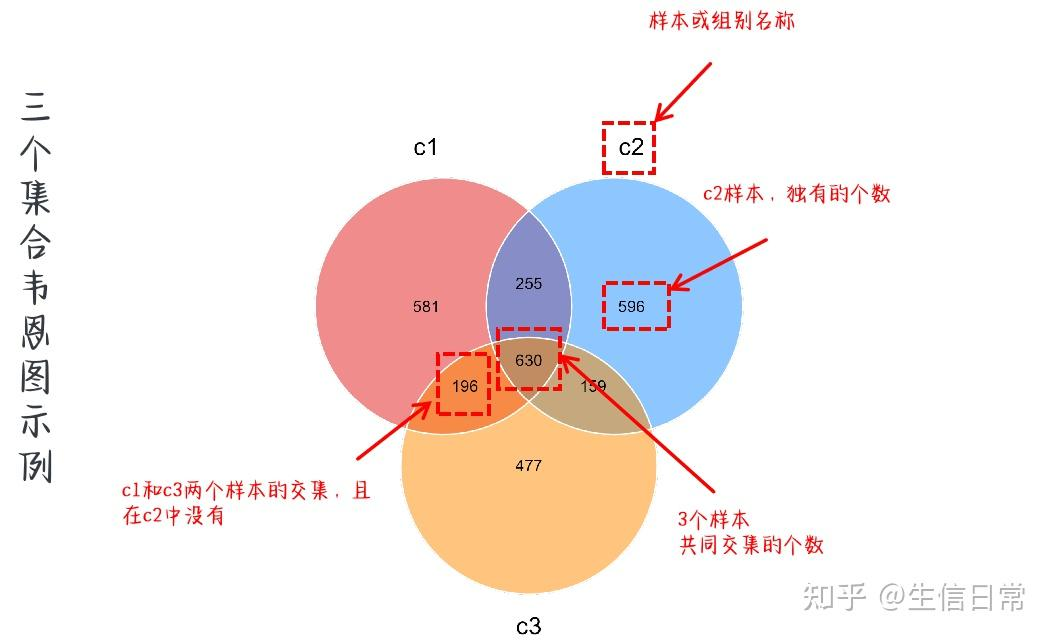
\includegraphics[width=0.6\textwidth]{Venn_Graphic.jpg}
    \caption{Venn 图示例}
    \label{fig:venn_diagram}
\end{figure}

%\nocite{*}
%\bibliography{ref}
\end{document}